\documentclass{article}
\usepackage[latin1]{inputenc}
\usepackage{graphicx}
\usepackage{a4wide}
\usepackage[colorlinks,linkcolor=blue]{hyperref}

\renewcommand{\ref}[1]{\link{\htmlref{#1}}{#1}}
\newcommand{\reffun}[1]{{\tt #1} (\ref{sec:#1})}
\newcommand{\tab}{\hspace{5mm}}
\newcommand{\hide}[1]{}

\title{SkyBotiX: Micro Helicopter API}
\author{C\'edric Pradalier}
\begin{document}
\maketitle

\section{Introduction}
\label{sec:intro}
This document proposes an API for an easy to use micro-helicopter. The
application context here is to have a host computer communicating with the
micro-helicopter in order to send it high level commands. Communication has
been tested on bluetooth, but other medium can be considered. 

Most important, this has been written from a user point of view: it shows what
I think a user would expect, without taking into account the reality of the
controller implementation. .

\subsection{Typical program 1: basic monitoring}
\begin{verbatim}
Connect
Do forever {
    Request helicopter state
    Display helicopter state
}
\end{verbatim}

\subsection{Typical program 2: basic control}
\begin{verbatim}
Connect
Do forever {
    Request helicopter state
    Compute control using state
    Send control commands
}
\end{verbatim}

\subsection{Typical program 3: advanced monitoring}
\begin{verbatim}
Connect
Configure communication channels for continous streaming
Do forever {
    Receive helicopter state
}
\end{verbatim}

\subsection{Typical program 4: advanced remote control}
\begin{verbatim}
Connect
Configure communication channels for continuous streaming
Do forever {
    Receive helicopter state
    Compute control
    Send control commands
}
\end{verbatim}

\section{General Remarks}
The API provides 3 layers of increasing complexity:
\begin{itemize}
\item Simplified, defined in {\tt sbsimple.h} provides a default initialisation
function, and only the basic function for doing sensor-based servoing. 
\item Complete, defined in {\tt sbapi.h} provides access to all the helicopter
configuration functions and controls, including raw commands. 
\item Raw communication channels, defined in {\tt sbchannel.h}, used to send
message directly to the helicopter. 
\end{itemize}


\subsection{struct SBControlContext}
\label{sec:structSBControlContext}
This C structure contains all the information relative to the communication
channel and the reception of data. It should be used as an abstract type,
without relying on a specific implementation of its content.

All functions in complete API take as arguments a pointer on a SBControlContext
struct. Initialisation functions fill in the required contents. 

\subsection{struct SBApiSimpleContext}
\label{sec:structSBApiSimpleContext}
This C structure contains an instance of SBControlContext, plus numerous useful
variables to control the execution of a basic control loop. In particular, it
stores information about the data reception thread used to listen for
helicopter messages.

An important object in the SBApiSimpleContext structure is state. This is
updated each time a new data packet is received from the helicopter. 

All functions in the simplified API take as arguments a pointer on a
SBApiSimpleContext struct. Initialisation functions fill in the required contents. 

\subsection{Return values}
\label{sec:returnValues}
All the functions of this API return 0 on success and anything else on failure. 
Error codes are not fully documented yet, but shoud follow the unix errno
semantic whenever possible. 

\section{The simplified API}

\subsection{sbSimpleDefaultContext}
\label{sec:sbSimpleDefaultContext}
\begin{verbatim}
int sbSimpleDefaultContext(SBApiSimpleContext *context);
\end{verbatim}
Initialise the context with default values. Should be called before any 
use of the context variable 

\subsection{sbSimpleInitialise}
\label{sec:sbSimpleInitialise}
\begin{verbatim}
int sbSimpleInitialise(SBApiSimpleContext *context);
\end{verbatim}
Initialise the communication, the helicopter and possibly the 
state reception thread, based on the information in context.
All configuration options are only read during this stage.


\subsection{sbSimpleReachNavState}
\label{sec:sbSimpleReachNavState}
\begin{verbatim}
int sbSimpleReachNavState(SBApiSimpleContext *context, 
		int desired, double timeout_sec);
\end{verbatim}

Reach the desired navigation state within timeout\_sec. If several
intermediary state are required, they will be reached one by one.

\subsection{sbSimpleTerminate}
\label{sec:sbSimpleTerminate}
\begin{verbatim}
int sbSimpleTerminate(SBApiSimpleContext *context);
\end{verbatim}
Terminate the connection to the helicopter and bring it to a safe
configuration (landed, motor stopped)

\subsection{sbSimpleWaitState}
\label{sec:sbSimpleWaitState}
\begin{verbatim}
int sbSimpleWaitState(SBApiSimpleContext *context, SBHeliState *state, 
        double timeout_sec);
\end{verbatim}

Wait for a new state to be received. Only make sense in continuous 
communication mode. If state is not null, the received state is copied
inside. If it is null, it is only copied in the internal storage, and in 
context->stateP pointer if not null


\subsection{sbSimpleControl}
\label{sec:sbSimpleControl}
\begin{verbatim}
int sbSimpleControl(SBApiSimpleContext *context, 
        double roll, double pitch, double yaw,
        double altitude);
\end{verbatim}

Send a control command to the helicopter. The meaning of the command
depends on the control mode configuration at initialisation, if not changed
with sbConfigureControl


\subsection{sbSimpleRawControl}
\label{sec:sbSimpleRawControl}
\begin{verbatim}
int sbSimpleRawControl(SBApiSimpleContext *context, 
        double motor1, double motor2, double servo1, double servo2);
\end{verbatim}

Send a raw control command to the helicopter. Only work in RAW\_COMMAND
control mode



\section{Connection functions}
\label{sec:connection}
\subsection{sbOpenSerialCommunication}
\label{sec:sbOpenSerialCommunication}
\begin{verbatim}
int sbOpenSerialCommunication(struct SBControlContext *control,
        const char *device, unsigned int baudrate);
\end{verbatim}
This function opens a serial communication channel to the helicopter. 
Under linux, device may be (for instance) {\tt /dev/tty0} or {\tt /dev/rfcomm0} for
bluetooth, and baudrate is a define symbol as defined in bit/termios.h (e.g.
B115200). 

\subsection{sbOpenSocketCommunication}
\label{sec:sbOpenSocketCommunication}
\begin{verbatim}
int sbOpenSocketCommunication(struct SBControlContext *control,
        const char *hostname, unsigned int port);
\end{verbatim}
This function opens a network communication channel to the helicopter.
This may be used in simulation or possibly to communicate via an on-board
network-enabled processor. Argument hostname is the hostname or IP of the
destination host and port is the UDP port of the communication.

Currently, there is no server responding to this communication request.

\subsection{sbCloseCommunication}
\label{sec:sbCloseCommunication}
\begin{verbatim}
int sbCloseCommunication(struct SBControlContext *control);
\end{verbatim}
Closes the communication channel and release any resource if required.

\subsection{sbLockCommunication}
\label{sec:sbLockCommunication}
\begin{verbatim}
int sbLockCommunication(struct SBControlContext *control);
\end{verbatim}
Locks the communication channel to prevent concurrent access from different
threads. Currently, this will only work on POSIX systems.

\subsection{sbUnlockCommunication}
\label{sec:sbUnlockCommunication}
\begin{verbatim}
int sbUnlockCommunication(struct SBControlContext *control);
\end{verbatim}
Unlocks the communication channel

\subsection{sbConnect}
\label{sec:sbConnect}
\begin{verbatim}
int sbConnect(struct SBControlContext *control);
\end{verbatim}
This function is seen as a placeholder for the connection mechanism to the
helicopter. In current implementation, if the connection has been established
correctly, it always returns successfully.

Future implementation may change the behaviour.

\subsection{sbDisconnect}
\label{sec:sbDisconnect}
\begin{verbatim}
int sbDisconnect(struct SBControlContext *control);
\end{verbatim}
When (and if) a proper connection mechanism is designed, then this function
will perform the disconnection from the platform.

\section{Configuration fonctions}
\label{sec:configuration}
\subsection{sbConfigureOAMode}
\label{sec:sbConfigureOAMode}
\begin{verbatim}
int sbConfigureOAMode(struct SBControlContext *control, unsigned int oavoidMode);
\end{verbatim}
Configures the obstacle avoidance behavior on the helicopter.
{\em oavoidMode} describes the obstacle avoidance behavior using flags defined
in {\tt sbconst.h}:
\begin{itemize}
\item SB\_OA\_NONE: no obstacle avoidance.
\item SB\_OA\_VERTICAL: only vertical obstacle avoidance, using downward
looking range sensor.
\item SB\_OA\_HORIZONTAL: only horizontal obstacle avoidance, using horizontal
range sensors if available.
\item A OR of the above to combine the behaviors.
\end{itemize}

\subsection{sbConfigureComm}
\label{sec:sbConfigureComm}
\begin{verbatim}
int sbConfigureComm(struct SBControlContext *control, 
        unsigned int commMode,
        unsigned int frequency,
        unsigned long contents);
\end{verbatim}
Configures the communication behavior, in particular if the controlling computer
will access the helicopter state via polling or receive it at fixed frequency.
{\em commMode} is set using a flag defined from {\tt sbconst.h}. It can be:
\begin{itemize}
\item SB\_COM\_ONREQUEST: the helicopter state is only sent when requested with
sbRequestState. Arguments frequency and contents are ignored.
\item SB\_COM\_CONTINUOUS: the helicopter will send its state continuously,
{\em frequency} time per second. Only state variable flagged in {\em contents}
(see section \ref{sec:state} on state) will be sent. Maximum frequency
achievable on a bluetooth link depends on the number of state item requested,
and how often the communication direction is switched. Values between 10 and
200 seem possible.
\end{itemize}

\subsection{sbConfigureControl}
\label{sec:sbConfigureControl}
\begin{verbatim}
int sbConfigureControl(struct SBControlContext *control, 
        unsigned int roll,
        unsigned int pitch,
        unsigned int yaw,
        unsigned int altitude,
        unsigned int horizontal);
\end{verbatim}
Configures the individual axis control modes. Each axis can be controlled
either in position (SB\_CTRL\_POS), velocity (SB\_CTRL\_VEL) or relative 
displacement (SB\_CTRL\_REL), or not controlled (SB\_CTRL\_NONE). 
Not all modes apply to all axis, and some axis are coupled, preventing some
control to be requested simultaneously.   
Control modes are defined {\tt sbconst.h}.

Acceptable control (currently implemented/foreseen) are as follows:
\begin{itemize}
\item Roll: Position control only, Horizontal control is not possible
\item Pitch: Position control only, Horizontal control is not possible
\item Yaw (eq. Heading): Position and Velocity control
\item Altitude: Position and Velocity control
\item Horizontal: Velocity only, Roll and Pitch control is not possible
\end{itemize}

\subsection{sbConfigureTimeout}
\label{sec:sbConfigureTimeout}
\begin{verbatim}
int sbConfigureTimeout(struct SBControlContext *control, 
        unsigned short control_timeout_ms,
        unsigned short watchdog_timeout_ms);
\end{verbatim}
Configures the timeout policy for the control and general communication
watchdog. For both timeout, a value of zero does not change the current
setting. A value of 0xFFFF disactivate the timeout.  The control timeout is
used only when the navigation mode (see section \ref{sec:control} on controls) is
SB\_NAV\_CTRLLED.  In this case, if the controlling application does not issue
commands within the timeout, the helicopter automatically switch back to
SB\_NAV\_HOVER (constant height, constant yaw).

The watchdog timeout is used at any time, but really only makes sense when the
helicopter is controlled or hovering (i.e. in modes SB\_NAV\_CTRLLED and
SB\_NAV\_HOVER). In these mode, if no \reffun{sbSetNavMode} request are
received within the timeout, the system automatically switch to SB\_NAV\_SINK
(constant heading and slowly decreasing altitude until touch down).  This
watchdog is useful to implement a safe behavior in case the communication link
gets broken.

\section{Control functions}
\label{sec:control}
\subsection{sbSetNavMode}
\label{sec:sbSetNavMode}
\begin{verbatim}
int sbSetNavMode(struct SBControlContext *control, 
        unsigned int navmode);
\end{verbatim}
Set the navigation mode, with {\em navMode} as a flag defined in {\tt sbconst.h}.
The semantic of navigation mode is as follows:
\begin{itemize}
\item SB\_NAV\_STOP: the helicopter is stopped, on the ground, rotors stopped.
\item SB\_NAV\_IDLE: the helicopter is on the ground, rotors rotating but not enough
    for taking off.
\item SB\_NAV\_TAKEOFF: the helicopter takes off, and transition to
    SB\_NAV\_HOVER when take off succeeded.
\item SB\_NAV\_HOVER: the helicopter stays at constant height and yaw angle,
with no pitch or roll. No horizontal stabilisation is active.  If a watchdog is
active, and no {\tt sbSetNavMode} request is received after this timeout, the
helicopter transition to SB\_NAV\_SINK.
\item SB\_NAV\_LAND: the helicopter comes to the ground, and transition to
    SB\_NAV\_IDLE automatically after touch down.
\item SB\_NAV\_CTRLLED: the helicopter is ready to receive user commands using
  \reffun{sbSetControl}. If a control timeout is active, and no control is received 
  after this timeout, then the helicopter goes back to SB\_NAV\_HOVER.
\end{itemize}
{\tt sbSetNavMode} is also used as a keep-alive function, indicating that the
controlling process is still active, and as a result, should be called
regularly (at least once per second with the default settings). See
\reffun{sbConfigureTimeout} for more details.

A detailed explanation of mode transition is given in appendix~\ref{sec:modes}.

\subsection{sbSetControl}
\label{sec:sbSetControl}
\begin{verbatim}
int sbSetControl(struct SBControlContext *control, 
        double roll, double pitch, double yaw,
        double altitude, double hx, double hy);
\end{verbatim}
Gives the set-points of the helicopter control laws. The semantic of the
set-point depends of the control modes defined with
\reffun{sbConfigureControl}.  Command clipping may be implemented, depending on
the helicopter platform.
If obstacle avoidance is active, it may also take precedence over requested
control. 
Control axis where the control mode has been configured to
SB\_CTRL\_NONE can be set to any value (0 is recommended).

Only International System units are used in this function: rad, rad/s, m, m/s


\section{State functions}
\label{sec:state}

\begin{table}
\centering
\begin{tabular}{|l|p{0.6\columnwidth}|}
\hline
Content flag & Semantic \\
\hline
\hline
SBS\_MODES         & System mode set using the configuration function
    (\ref{sec:configuration}):navigation state, communication mode, control
    modes, obstacle avoidance. \\
\hline
SBS\_TIMESTAMP     & System timestamp. \\
\hline
SBS\_RPY         & Roll, pitch, yaw from IMU. \\
\hline
SBS\_GYRO         & Roll, pitch, yaw rate from IMU. \\
\hline
SBS\_ACCEL         & Acceleration from IMU. \\
\hline
SBS\_MAGNETO     & Magnetic field vector from IMU. \\
\hline
SBS\_IMUTEMP     & Temperature from IMU. \\
\hline
SBS\_ZRANGE         & Range to the floor or nearest obstacle downward. \\
\hline
SBS\_ZPRESSURE     & Altitude from pressure sensor. \\
\hline
SBS\_HRANGES     & Horizontal ranges to obstacles. \\
\hline
SBS\_XY\_REL     & Distance to closest object. \\
\hline
SBS\_BATTERY     & Battery status. \\
\hline
SBS\_TIMEOUT     & Timeout currently used, configured using
    \reffun{sbConfigureTimeout}. \\
\hline
SBS\_O\_ATTITUDE & Output of Attitude control. \\
\hline
SBS\_O\_ALTITUDE & Output of Altitude control. \\
\hline
SBS\_O\_TOL         & Output of TakeOff/Landing control. \\
\hline
SBS\_O\_XY         & Output of XY control. \\
\hline
SBS\_O\_OAVOID     & Output of Obstacle avoidance control. \\
\hline
\hline

Combined flags & for convenience \\
\hline
SBS\_ALL              & All of the above. \\
\hline
SBS\_IMU\_ALL          &  All the IMU data. \\
\hline
SBS\_RANGES\_ALL      &  All the ranges data. \\
\hline
SBS\_ALTITUDE\_ALL  &  All the altitude data (pressure and range). \\
\hline
SBS\_OUTPUT\_ALL      &  All the controller output. \\
\hline
\end{tabular}
\caption{Data selection flags for skybotics platform communication}
\label{table:contents}
\end{table}

\subsection{sbGetSensorList}
\label{sec:sbGetSensorList}
\begin{verbatim}
int sbGetSensorList(struct SBControlContext *control, unsigned long *list);
\end{verbatim}
This functions returns the list of sensing modalities implemented on this
platform. The output is returned in {\em list} under the form of a OR'ed mask
of flags used to request helicopter state (see table~\ref{table:contents}).
This mask can then be used with a AND operator when requesting the helicopter
state, in order to request only relevant data.

\subsection{sbRequestState}
\label{sec:sbRequestState}
\begin{verbatim}
int sbRequestState(struct SBControlContext *control,
        unsigned long contents, SBHeliState *state);
\end{verbatim}
Requests the helicopter state. {\em contents} is a OR'ed mask of flags defined
in table~\ref{table:contents}. Only the relevant fields of {\em state} are
modified by the function. A detailed description of the SBHeliState type is
given in table~\ref{table:SBHeliState}.

This function can be used even when the communication mode
is continuous (see \ref{sec:sbConfigureComm}), for instance, to request
different data from time to time.  Given that changing communication direction
is very costly with bluetooth, it may be better to just augment the number of
requested item in continuous mode.

\subsection{sbReceiveState}
\label{sec:sbReceiveState}
\begin{verbatim}
int sbReceiveState(struct SBControlContext *control,SBHeliState *state,
        unsigned int timeout_ms);
\end{verbatim}
Receives a state message, as specified in sbConfigureComm.  {\em timeout\_ms}
represent a timeout (in ms) for the reception of messages. A value of zero
implies an infinite wait. On success, the field of {\em state} specified in the
{\em contents} argument of \reffun{sbConfigureComm} are updated.

\subsection{sbRegisterStateCallback}
\label{sec:sbRegisterStateCallback}
\begin{verbatim}
int sbRegisterStateCallback(struct SBControlContext *control, 
    void (*stateCallback)(SBHeliState *state, void *userData),
    void *userData);
\end{verbatim}
This function illustrates the spirit of this API.  At any one time, only one
process/thread should use the communication channel. 
In synchronous mode, the dialogue is only question/response, but 
when the communication is continuous, the helicopter may send state
information at any time. When a question/response mode (control, configuration)
is started, some state information may arrive after the question. while waiting
for the answer. This callback can be setup to handle this piece of data in this
case, instead of discarding it.  Figure~\ref{fig:callback} illustrates a
possible use of this function.

In practice, each time a question/response interaction is started, if a state
message is received while waiting for the response, then {\em stateCallback} is
called with the decoded {\em state} and the pointer {\em userData} used when
registering the callback.

\begin{figure}[htbp]
\begin{verbatim}
 // Global variable to store the state, for illustration
 SBHeliState state;
 void * receive_thread(void *) {
     ...
         while (1) {
             sbLockCommunication(&control);
             sbReceiveState(control,&state);
             sbUnlockCommunication(&control);
         }
     ...
 }

 void recCB(SBHeliState *rstate, void *user_data) {
     memcpy(&state,&rstate,sizeof(SBHeliState);
 }
 
 int main() {
     struct SBControlContext control;
     
     sbOpenSerialCommunication(&control,"/dev/rfcomm0",B115200)
     sbConnect(&control);
     sbRegisterStateCallback(&control,recCB,NULL);
     sbConfigureComm(SB_COM_CONTINUOUS,30,SBS_RPY | SBS_ZRANGES);

     start receive_thread()

     while (1) {
         wait something
         sbLockCommunication(&control);
         // Any state received here will be handle by the callback
         sbSetNavMode(&control,SB_NAV_HOVER);
         sbUnlockCommunication(&control);
     }
     sbDisconnect(&control);
     ...
 }
\end{verbatim}
\caption{Example of program illustrating the use of the state reception
callback.}
\label{fig:callback}
\end{figure}


\begin{table}[htbp]
\begin{tabular}{|lp{0.6\columnwidth}|}
\hline
C Structure & State flags from table~\ref{table:contents} and details \\
\hline
typedef struct  \{ & \\
\tab    unsigned char errorFlags; & Always included \\
\tab    unsigned long content; & Always included.
    Use a AND of the state content flags (table~\ref{table:contents})
    SBS\_\dots flags above to check the content, e.g:
\begin{verbatim}
if (state.content & SBS_RPY) {
    compute_odo(state.roll,state.pitch,state.yaw);
}
\end{verbatim}
    This content should correspond to what has been configured in
    \reffun{sbConfigureComm} or requested in \reffun{sbRequestState} \\
\tab    unsigned long timeStamp; & SBS\_TIMESTAMP, timestamp in ms, from helicopter
    startup.\\
\tab    unsigned short controlTimeout; & SBS\_TIMEOUT, as configured with
    \reffun{sbConfigureTimeout}.\\
\tab    unsigned short watchdogTimeout; & SBS\_TIMEOUT, as configured with
    \reffun{sbConfigureTimeout}.\\
\tab    struct \{ & SBS\_MODES\\
\tab \tab        unsigned char navigation; & as set with \reffun{sbSetNavMode}.\\
\tab \tab        unsigned char communication; & as set with
    \reffun{sbConfigureComm}. \\
\tab \tab        unsigned char oavoid; & as set with \reffun{sbConfigureOAMode}.\\
\tab \tab        unsigned char rollAxis; & as set with \reffun{sbConfigureControl}, when in SB\_NAV\_CTRLLED mode.\\
\tab \tab        unsigned char pitchAxis; & idem.\\
\tab \tab        unsigned char yawAxis; & idem.\\
\tab \tab        unsigned char altAxis; & idem.\\
\tab \tab        unsigned char horizAxis; & idem.\\
\tab    \} mode; & \\
\tab
\tab    float roll, pitch, yaw; & SBS\_RPY, from IMU.\\
\tab    float gyro[3]; & SBS\_GYRO, from IMU.\\
\tab    float accel[3]; & SBS\_ACCEL, from IMU.\\
\tab    float magneto[3]; & SBS\_MAGNETO, from IMU.\\
\tab    float imutemp; & SBS\_IMUTEMP, from IMU.\\
\tab    float zrange; & SBS\_ZRANGE, from downward looking range sensor.\\ 
\tab    float zpressure; & SBS\_ZPRESSURE\\
\tab    float hranges[3]; & SBS\_HRANGES, from horizontal range sensors. \\
\tab    float xrel, yrel; & SBS\_XY\_REL, distance to closest object, computed
    from range sensors.\\
\tab    float battery; & SBS\_BATTERY\\
\tab    unsigned short o\_attitude[3]; & SBS\_O\_ATTITUDE, semantic TBD\\
\tab    unsigned short o\_altitude; & SBS\_O\_ALTITUDE, semantic TBD\\
\tab    unsigned short o\_tol; & SBS\_O\_TOL, semantic TBD\\
\tab    unsigned short o\_xy[2]; & SBS\_O\_XY, semantic TBD\\
\tab    unsigned short o\_oavoid[2]; & SBS\_O\_OAVOID, semantic TBD\\
\} SBHeliState; & \\
\hline
\end{tabular}
\caption{Description of C structure {\tt SBHeliState}. Only International System unit used here: rad, rad/s, m, m/s}
\label{table:SBHeliState}
\end{table}
        

\newpage
\appendix

\section{Navigation modes}
\label{sec:modes}
\begin{figure}[htb]
\centering
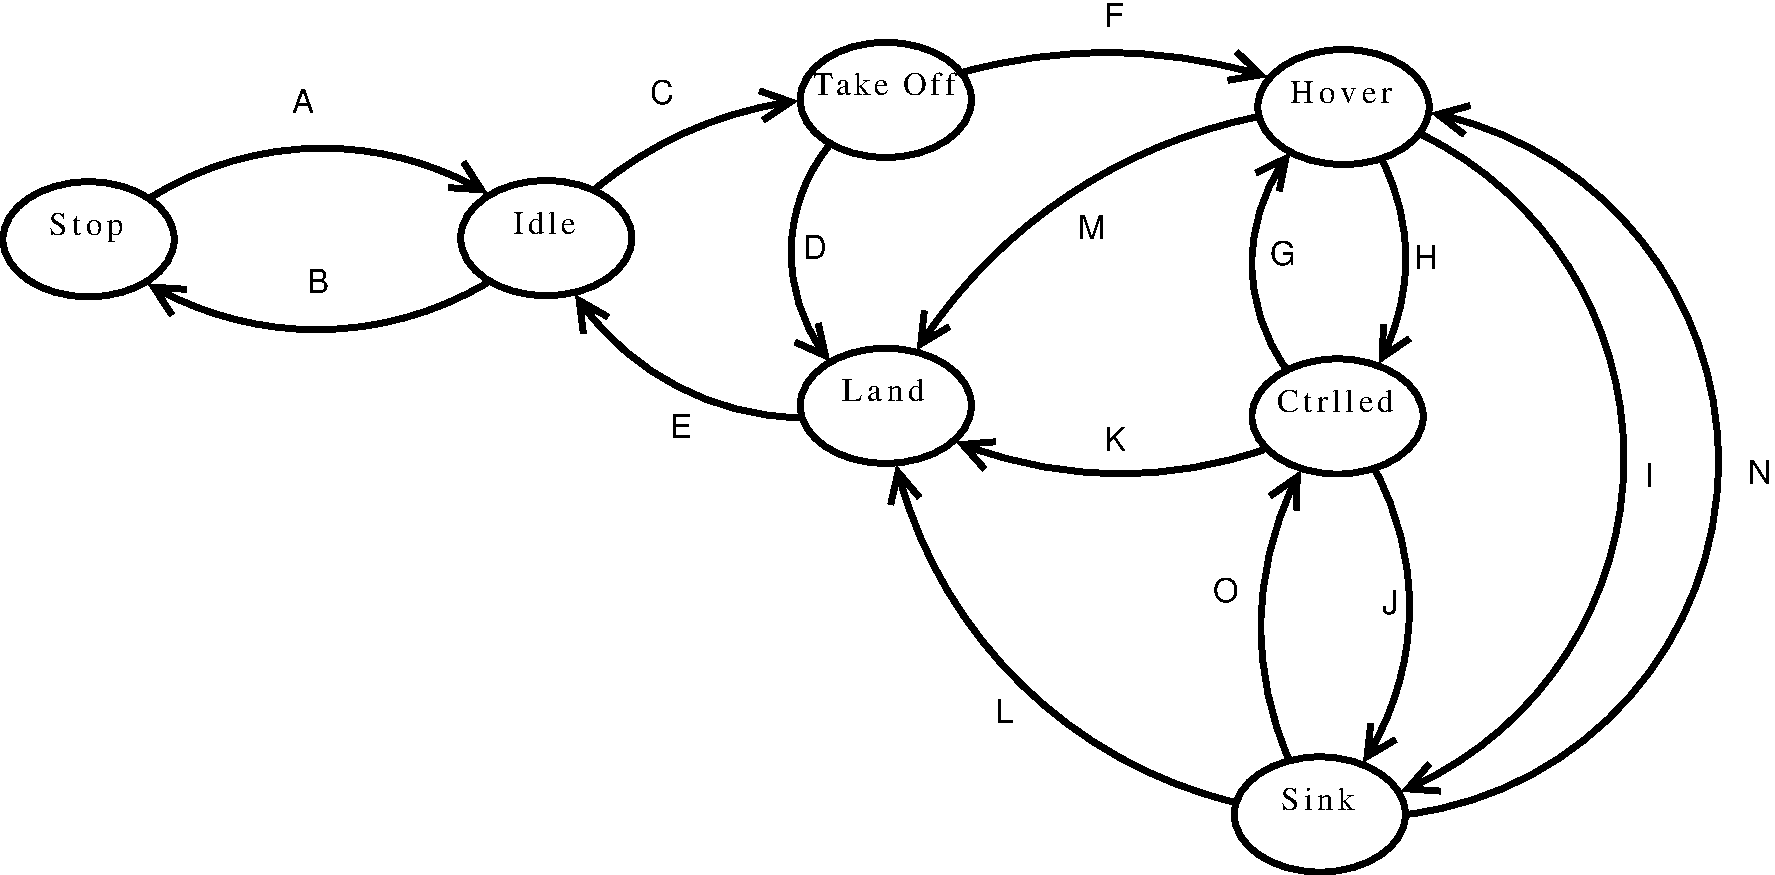
\includegraphics[width=0.9\columnwidth]{API_automaton}
\caption{MAV API: Envisaged control modes}
\label{fig:automaton}
\end{figure}
Figure \ref{fig:automaton} is a state automaton showing the various behaviour
modes expected from a MAV. It is important to notice that these modes may be
virtual modes: they don't have to correspond to what is really implemented in
the controller, they describes various behaviours, semantically consistent and
with the same set of constraints. The remaining of this section details the
expected behaviour in each mode, the transition conditions and the accepted
commands.

For the safety of the MAV, it is assumed that a control watchdog is
implemented. This watchdog is triggered when the connection between the MAV and
the host computer is broken, or if the host controller stop sending control
commands. See section \ref{sec:usecases} for details.

\subsection{Stop}
\subsubsection{Description}
\begin{itemize}
\item System is checked up
\item All the motors are powered off
\item The pressure sensor reference is initialised
\end{itemize}
\subsubsection{Transition conditions}
\begin{description}
\item[Transition A]: on user request.
\end{description}
\subsubsection{Accepted commands}
\begin{itemize}
\item Set Mode to Idle
\end{itemize}

\subsection{Idle}
\subsubsection{Description}
\begin{itemize}
\item All systems powered on
\item All motors rotating slowly
\end{itemize}
\subsubsection{Transition conditions}
\begin{description}
\item[Transition B]: on user request or on watchdog timeout
\item[Transition C]: on user request: mode set to Take Off or Hover
\end{description}
\subsubsection{Accepted commands}
\begin{itemize}
\item Set Mode to Stop, Take Off or Hover
\end{itemize}

\subsection{Take Off}
\subsubsection{Description}
\begin{itemize}
\item The MAV stabilise itself to hovering at 10cm above ground (TBC), based on
pressure sensor. The resulting displacement is relative.
\end{itemize}
\subsubsection{Transition conditions}
\begin{description}
\item[Transition F]: the system is stable at the required height.
\item[Transition D]: on user request, watchdog timeout, action timeout or exception.
\end{description}
\subsubsection{Accepted commands}
\begin{itemize}
\item Set Mode to Land
\end{itemize}

\subsection{Land}
\subsubsection{Description}
\begin{itemize}
\item Bring the MAV to touch down. Downward range sensor is used to estimate
touch down. The maximum velocity downward is XX (TBD). 
\end{itemize}
\subsubsection{Transition conditions}
\begin{description}
\item[Transition E]: Contact has been detected.
\end{description}
\subsubsection{Accepted commands}
\begin{itemize}
\item None
\end{itemize}

\subsection{Hover}
\subsubsection{Description}
\begin{itemize}
\item Yaw and altitude are kept constant, roll and pitch kept to zero. The MAV
will certainly be drifting in this mode.
\item If available, the horizontal obstacle avoidance is active.
\item Downward obstacle avoidance is active
\item Data fusion for altitude estimation is active. 
\end{itemize}
\subsubsection{Transition conditions}
\begin{description}
\item[Transition H]: on user request
\item[Transition I]: on watchdog timeout
\item[Transition M]: on user request
\end{description}
\subsubsection{Accepted commands}
\begin{itemize}
\item Set Mode to Land
\item Set Mode to Controlled
\end{itemize}

\subsection{Controlled -- Ctrlled}
\subsubsection{Description}
\begin{itemize}
\item Altitude, yaw and position are controlled as requested
\item Downward obstacle avoidance may be activated
\item If available, horizontal obstacle avoidance may be activated
\end{itemize}
\subsubsection{Transition conditions}
\begin{description}
\item[Transition G]: on user request or on control timeout (i.e. the watchdog
has not been triggered, but no remote commands have been received).
\item[Transition J]: on watchdog timeout 
\item[Transition K]: on user request
\end{description}
\subsubsection{Accepted commands}
\begin{itemize}
\item Set Mode to Hover
\item Set Mode to Land
\item Desired altitude, yaw and horizontal controls. In position or rate as
available. 
\end{itemize}

\subsection{Sink}
\subsubsection{Description}
\begin{itemize}
\item Altitude is slowly controlled down (for instance 5cm/s) until touch down
\item Any desired control is ignored until the connection is reset (see section
\item If available, the horizontal obstacle avoidance is active.
\ref{sec:sbConfigureOAMode}).
\end{itemize}
\subsubsection{Transition conditions}
\begin{description}
\item[Transition N]: on user request after connection reset.
\item[Transition O]: on user request after connection reset.
\item[Transition L]: on user request after connection reset, or when the
distance to ground becomes smaller than 10cm (TBC).
\end{description}
\subsubsection{Accepted commands}
\begin{itemize}
\item Set Mode to Hover
\item Set Mode to Land
\item Set Mode to Controlled
\end{itemize}


\newpage
\section{Use Cases: from the programmer side}
\label{sec:usecases}
Several type of user programming can be foreseen. This section try to list them
all. Not all of them may be implementable.

\subsection{Considering only one helicopter}
\subsubsection{Polling, single thread}
\begin{tabbing}
\=\hspace{1cm}\=\hspace{6cm}\=\kill
Set Communication Mode to Polling\\
\>Forever:\\
\>\>Get MAV State\>{\it Polling}\\
\>\>Set Control Mode\>{\it Reset WatchDog}\\
\>\>Set Control \>{\it Z, Yaw, ...}
\end{tabbing}

\subsubsection{Polling, multi thread}
Set Communication Mode to Polling\\
\begin{tabular}{|l|l|}
\hline
Thread 1 & Thread 2 \\
\hline
\begin{minipage}{0.49\columnwidth}
\vspace{2mm}
Forever:\\
\hspace*{1cm}Get MAV State \\
\vspace{2mm}
\end{minipage} &
\begin{minipage}{0.49\columnwidth}
\vspace{2mm}
Forever:\\
\hspace*{1cm}Set Control Mode\\
\hspace*{1cm}Set Control\\
\vspace{2mm}
\end{minipage} \\
\hline
\end{tabular}

\subsubsection{Continuous, single thread}
\begin{tabbing}
\=\hspace{1cm}\=\hspace{6cm}\=\kill
\>Set Communication Mode to Continuous\\
\>Forever:\\
\>\>Receive MAV State\>{\it Server push}\\
\>\>Set Control Mode\>{\it Reset WatchDog}\\
\>\>Set Control \>{\it Z, Yaw, ...}
\end{tabbing}

\subsubsection{Continuous, multi thread}
Set Communication Mode to Continuous\\
\begin{tabular}{|l|l|}
\hline
Thread 1 & Thread 2 \\
\hline
\begin{minipage}{0.49\columnwidth}
\vspace{2mm}
Forever:\\
\hspace*{1cm}Receive MAV State \\
\vspace{2mm}
\end{minipage} &
\begin{minipage}{0.49\columnwidth}
\vspace{2mm}
Forever:\\
\hspace{1cm}Set Control Mode\\
\hspace*{1cm}Set Control\\
\vspace*{2mm}
\end{minipage} \\
\hline
\end{tabular}

\subsubsection{The video}
In addition to the above options, the video stream can also be polled or
received continuously, and it could (or should) be acquired in an independent
thread. 

\subsection{Considering several helicopter}
The type of MAV developed by SkyBotics are likely to be very suitable for
multi-UAV control. This should be taken into account when designing the API, so
that multiple UAV can be controlled from a single host computer. 


\end{document}

